%% BioMed_Central_Tex_Template_v1.06
%%                                      %
%  bmc_article.tex            ver: 1.06 %
%                                       %

%%IMPORTANT: do not delete the first line of this template
%%It must be present to enable the BMC Submission system to
%%recognise this template!!

%%%%%%%%%%%%%%%%%%%%%%%%%%%%%%%%%%%%%%%%%
%%                                     %%
%%  LaTeX template for BioMed Central  %%
%%     journal article submissions     %%
%%                                     %%
%%          <8 June 2012>              %%
%%                                     %%
%%                                     %%
%%%%%%%%%%%%%%%%%%%%%%%%%%%%%%%%%%%%%%%%%


%%%%%%%%%%%%%%%%%%%%%%%%%%%%%%%%%%%%%%%%%%%%%%%%%%%%%%%%%%%%%%%%%%%%%
%%                                                                 %%
%% For instructions on how to fill out this Tex template           %%
%% document please refer to Readme.html and the instructions for   %%
%% authors page on the biomed central website                      %%
%% http://www.biomedcentral.com/info/authors/                      %%
%%                                                                 %%
%% Please do not use \input{...} to include other tex files.       %%
%% Submit your LaTeX manuscript as one .tex document.              %%
%%                                                                 %%
%% All additional figures and files should be attached             %%
%% separately and not embedded in the \TeX\ document itself.       %%
%%                                                                 %%
%% BioMed Central currently use the MikTex distribution of         %%
%% TeX for Windows) of TeX and LaTeX.  This is available from      %%
%% http://www.miktex.org                                           %%
%%                                                                 %%
%%%%%%%%%%%%%%%%%%%%%%%%%%%%%%%%%%%%%%%%%%%%%%%%%%%%%%%%%%%%%%%%%%%%%

%%% additional documentclass options:
%  [doublespacing]
%  [linenumbers]   - put the line numbers on margins

%%% loading packages, author definitions

\documentclass[twocolumn]{bmcart}% uncomment this for twocolumn layout and comment line below
%\documentclass{bmcart}

%%% Load packages
%\usepackage{amsthm,amsmath}
%\RequirePackage{natbib}
%\RequirePackage[authoryear]{natbib}% uncomment this for author-year bibliography
%\RequirePackage{hyperref}
\usepackage[utf8]{inputenc} %unicode support
\usepackage[english]{babel}
\usepackage{graphicx}
\usepackage{tabularx}
\usepackage[citecolor=black, urlcolor=black,linkcolor=black]{hyperref}
\usepackage{amsmath}
%\usepackage[applemac]{inputenc} %applemac support if unicode package fails
%\usepackage[latin1]{inputenc} %UNIX support if unicode package fails


%%%%%%%%%%%%%%%%%%%%%%%%%%%%%%%%%%%%%%%%%%%%%%%%%
%%                                             %%
%%  If you wish to display your graphics for   %%
%%  your own use using includegraphic or       %%
%%  includegraphics, then comment out the      %%
%%  following two lines of code.               %%
%%  NB: These line *must* be included when     %%
%%  submitting to BMC.                         %%
%%  All figure files must be submitted as      %%
%%  separate graphics through the BMC          %%
%%  submission process, not included in the    %%
%%  submitted article.                         %%
%%                                             %%
%%%%%%%%%%%%%%%%%%%%%%%%%%%%%%%%%%%%%%%%%%%%%%%%%


%\def\includegraphic{}
%\def\includegraphics{}



%%% Put your definitions there:
\startlocaldefs
\endlocaldefs


%%% Begin ...
\begin{document}

%%% Start of article front matter
\begin{frontmatter}

\begin{fmbox}
\dochead{Report}

%%%%%%%%%%%%%%%%%%%%%%%%%%%%%%%%%%%%%%%%%%%%%%
%%                                          %%
%% Enter the title of your article here     %%
%%                                          %%
%%%%%%%%%%%%%%%%%%%%%%%%%%%%%%%%%%%%%%%%%%%%%%

\title{Alignment-free tools for metagenomics-data analysis}

%%%%%%%%%%%%%%%%%%%%%%%%%%%%%%%%%%%%%%%%%%%%%%
%%                                          %%
%% Enter the authors here                   %%
%%                                          %%
%% Specify information, if available,       %%
%% in the form:                             %%
%%   <key>={<id1>,<id2>}                    %%
%%   <key>=                                 %%
%% Comment or delete the keys which are     %%
%% not used. Repeat \author command as much %%
%% as required.                             %%
%%                                          %%
%%%%%%%%%%%%%%%%%%%%%%%%%%%%%%%%%%%%%%%%%%%%%%

\author[
   addressref={aff1},                   % id's of addresses, e.g. {aff1,aff2}
   corref={aff1},                       % id of corresponding address, if any
  % noteref={n1},                        % id's of article notes, if any
   email={robert.deibel@student.uni-tuebingen.de}   % email address
]{\inits{RD}\fnm{Robert} \snm{Deibel}}

%%%%%%%%%%%%%%%%%%%%%%%%%%%%%%%%%%%%%%%%%%%%%%
%%                                          %%
%% Enter the authors' addresses here        %%
%%                                          %%
%% Repeat \address commands as much as      %%
%% required.                                %%
%%                                          %%
%%%%%%%%%%%%%%%%%%%%%%%%%%%%%%%%%%%%%%%%%%%%%%

\address[id=aff1]{%                           % unique id
  \orgname{Eberhard-Karls Universität}, % university, etc
  %\street{Waterloo },                     %
  %\postcode{}                                % post or zip code
  \city{Tübingen},                              % city
  \cny{DE}                                    % country
}


%%%%%%%%%%%%%%%%%%%%%%%%%%%%%%%%%%%%%%%%%%%%%%
%%                                          %%
%% Enter short notes here                   %%
%%                                          %%
%% Short notes will be after addresses      %%
%% on first page.                           %%
%%                                          %%
%%%%%%%%%%%%%%%%%%%%%%%%%%%%%%%%%%%%%%%%%%%%%%

\begin{artnotes}
%\note{Sample of title note}     % note to the article
%\note[id=n1]{Equal contributor} % note, connected to author
\end{artnotes}

%\end{fmbox}% comment this for two column layout

%%%%%%%%%%%%%%%%%%%%%%%%%%%%%%%%%%%%%%%%%%%%%%
%%                                          %%
%% The Abstract begins here                 %%
%%                                          %%
%% Please refer to the Instructions for     %%
%% authors on http://www.biomedcentral.com  %%
%% and include the section headings         %%
%% accordingly for your article type.       %%
%%                                          %%
%%%%%%%%%%%%%%%%%%%%%%%%%%%%%%%%%%%%%%%%%%%%%%

\begin{abstractbox}

\begin{abstract} % abstract
	Metagenomics is the analysis of microorganisms of biotopes, like the human gut. 
	The high amount of reads obtained through NGS-methods as well as findings of unsequenced genomes in metagenominc data requires usage of lightweight tools independent of databases and alignment.
	In this report I introduce the two main branches of analysis tools, while setting the focus on alignment-free methods.\\
	While the alignment-based approaches align a target sequence against a database  -- as seen with Smith-Waterman or BLAST -- alignment-free methods have different approaches. Here I will showcase a selection of statistical and machine learning approaches.\\ 
	$D2z$, $Hao$ and $d_2^*$ are statistical approaches based on $k$-tupel count frequencies, similarity is measured by applying a metric and through interpretation with current biological knowledge.\\
	Usage of $k$-mers as vectors in high-dimensional space and BH-SNE visualizing related data in two dimensional scatter plots leads to an approach with high accuracy for simulated and real-world metagenomes alike.
	Especially for analysis of novel data, sampled from microbioms, alignment-free applications of metagenomics are essential for understanding the cooperation of microorganisms and for further research in immunology.
\end{abstract}

%%%%%%%%%%%%%%%%%%%%%%%%%%%%%%%%%%%%%%%%%%%%%%
%%                                          %%
%% The keywords begin here                  %%
%%                                          %%
%% Put each keyword in separate \kwd{}.     %%
%%                                          %%
%%%%%%%%%%%%%%%%%%%%%%%%%%%%%%%%%%%%%%%%%%%%%%

\begin{keyword}
\kwd{alignment-free}
\kwd{machine learning}
\kwd{statistic}
\kwd{metagenome}
\kwd{report}
\end{keyword}

% MSC classifications codes, if any
%\begin{keyword}[class=AMS]
%\kwd[Primary ]{}
%\kwd{}
%\kwd[; secondary ]{}
%\end{keyword}

\end{abstractbox}
%
\end{fmbox}% uncomment this for twcolumn layout

\end{frontmatter}

%%%%%%%%%%%%%%%%%%%%%%%%%%%%%%%%%%%%%%%%%%%%%%
%%                                          %%
%% The Main Body begins here                %%
%%                                          %%
%% Please refer to the instructions for     %%
%% authors on:                              %%
%% http://www.biomedcentral.com/info/authors%%
%% and include the section headings         %%
%% accordingly for your article type.       %%
%%                                          %%
%% See the Results and Discussion section   %%
%% for details on how to create sub-sections%%
%%                                          %%
%% use \cite{...} to cite references        %%
%%  \cite{koon} and                         %%
%%  \cite{oreg,khar,zvai,xjon,schn,pond}    %%
%%  \nocite{smith,marg,hunn,advi,koha,mouse}%%
%%                                          %%
%%%%%%%%%%%%%%%%%%%%%%%%%%%%%%%%%%%%%%%%%%%%%%

%%%%%%%%%%%%%%%%%%%%%%%%% start of article main body
% <put your article body there>
\section*{Introduction}
\subsection*{Metagenomics}
\paragraph*{A puddle of mud}
The metagenome is the whole set of transcripts of a population of microorganisms in a microbiome sample. Metagenomics is the study and analysis of these metagenomes \cite{handelsman2004metagenomics}.\\
A microbiome consists of countless bacteria, archea and viruses; out of which $>$90\% are uncultureable, using sequencing and metagenomic analysis as a way to study these.\\
Metagenomics is used in the design of antibiotics and medicine or to analyze the metabolism of microorganisms, making it a rapidly developing field of research.
%\paragraph*{Accumulated data from microbiome samples}

%Choosing a sample is the easiest part of the analysis of a microbiome; the following steps are:\\
%\begin{enumerate}
%	\item DNA isolation from samples
%	\item construction of DNA libraries (typically in \textit{E. Coli} as host)
%	\item Mining for clones and DNA sequences of interest
%	\item Accumulation of desired clones and DNA sequences
%\end{enumerate}
%as stated in Streit \textit{et al.} \cite{STREIT2004492}, to obtain a metagenomic library, which is the base of analysis.\\
\paragraph*{NGS -- Next Generation Sequencing}
Advances in sequencing made metagenomics as a field possible.
Nowadays new high throughput methods, also Next Generation Sequencing or NGS for short, are used to generate comparable data from real-world samples. NGS is a term for methods of rapid parallelized sequencing, producing thousands or millions of reads concurrently.\\
 Data analysis can the be carried out on these reads.
\paragraph*{Goals}
Metagenomics-data, analyzed through align\-ment-free methods, allows insight into the ways of a broad spectrum of  microorganismal life. Differing from the classical approach of alignment, where newly found sequences are often unanalyzed, these alignment-free methods could provide first evidence of origin and function on novel sequences.\\
In this report, I want to state two branches of metagenomic analysis, while focusing on alignment-free methods. State different approaches, the strengths and weaknesses.
%\begin{figure}
%	\centering
%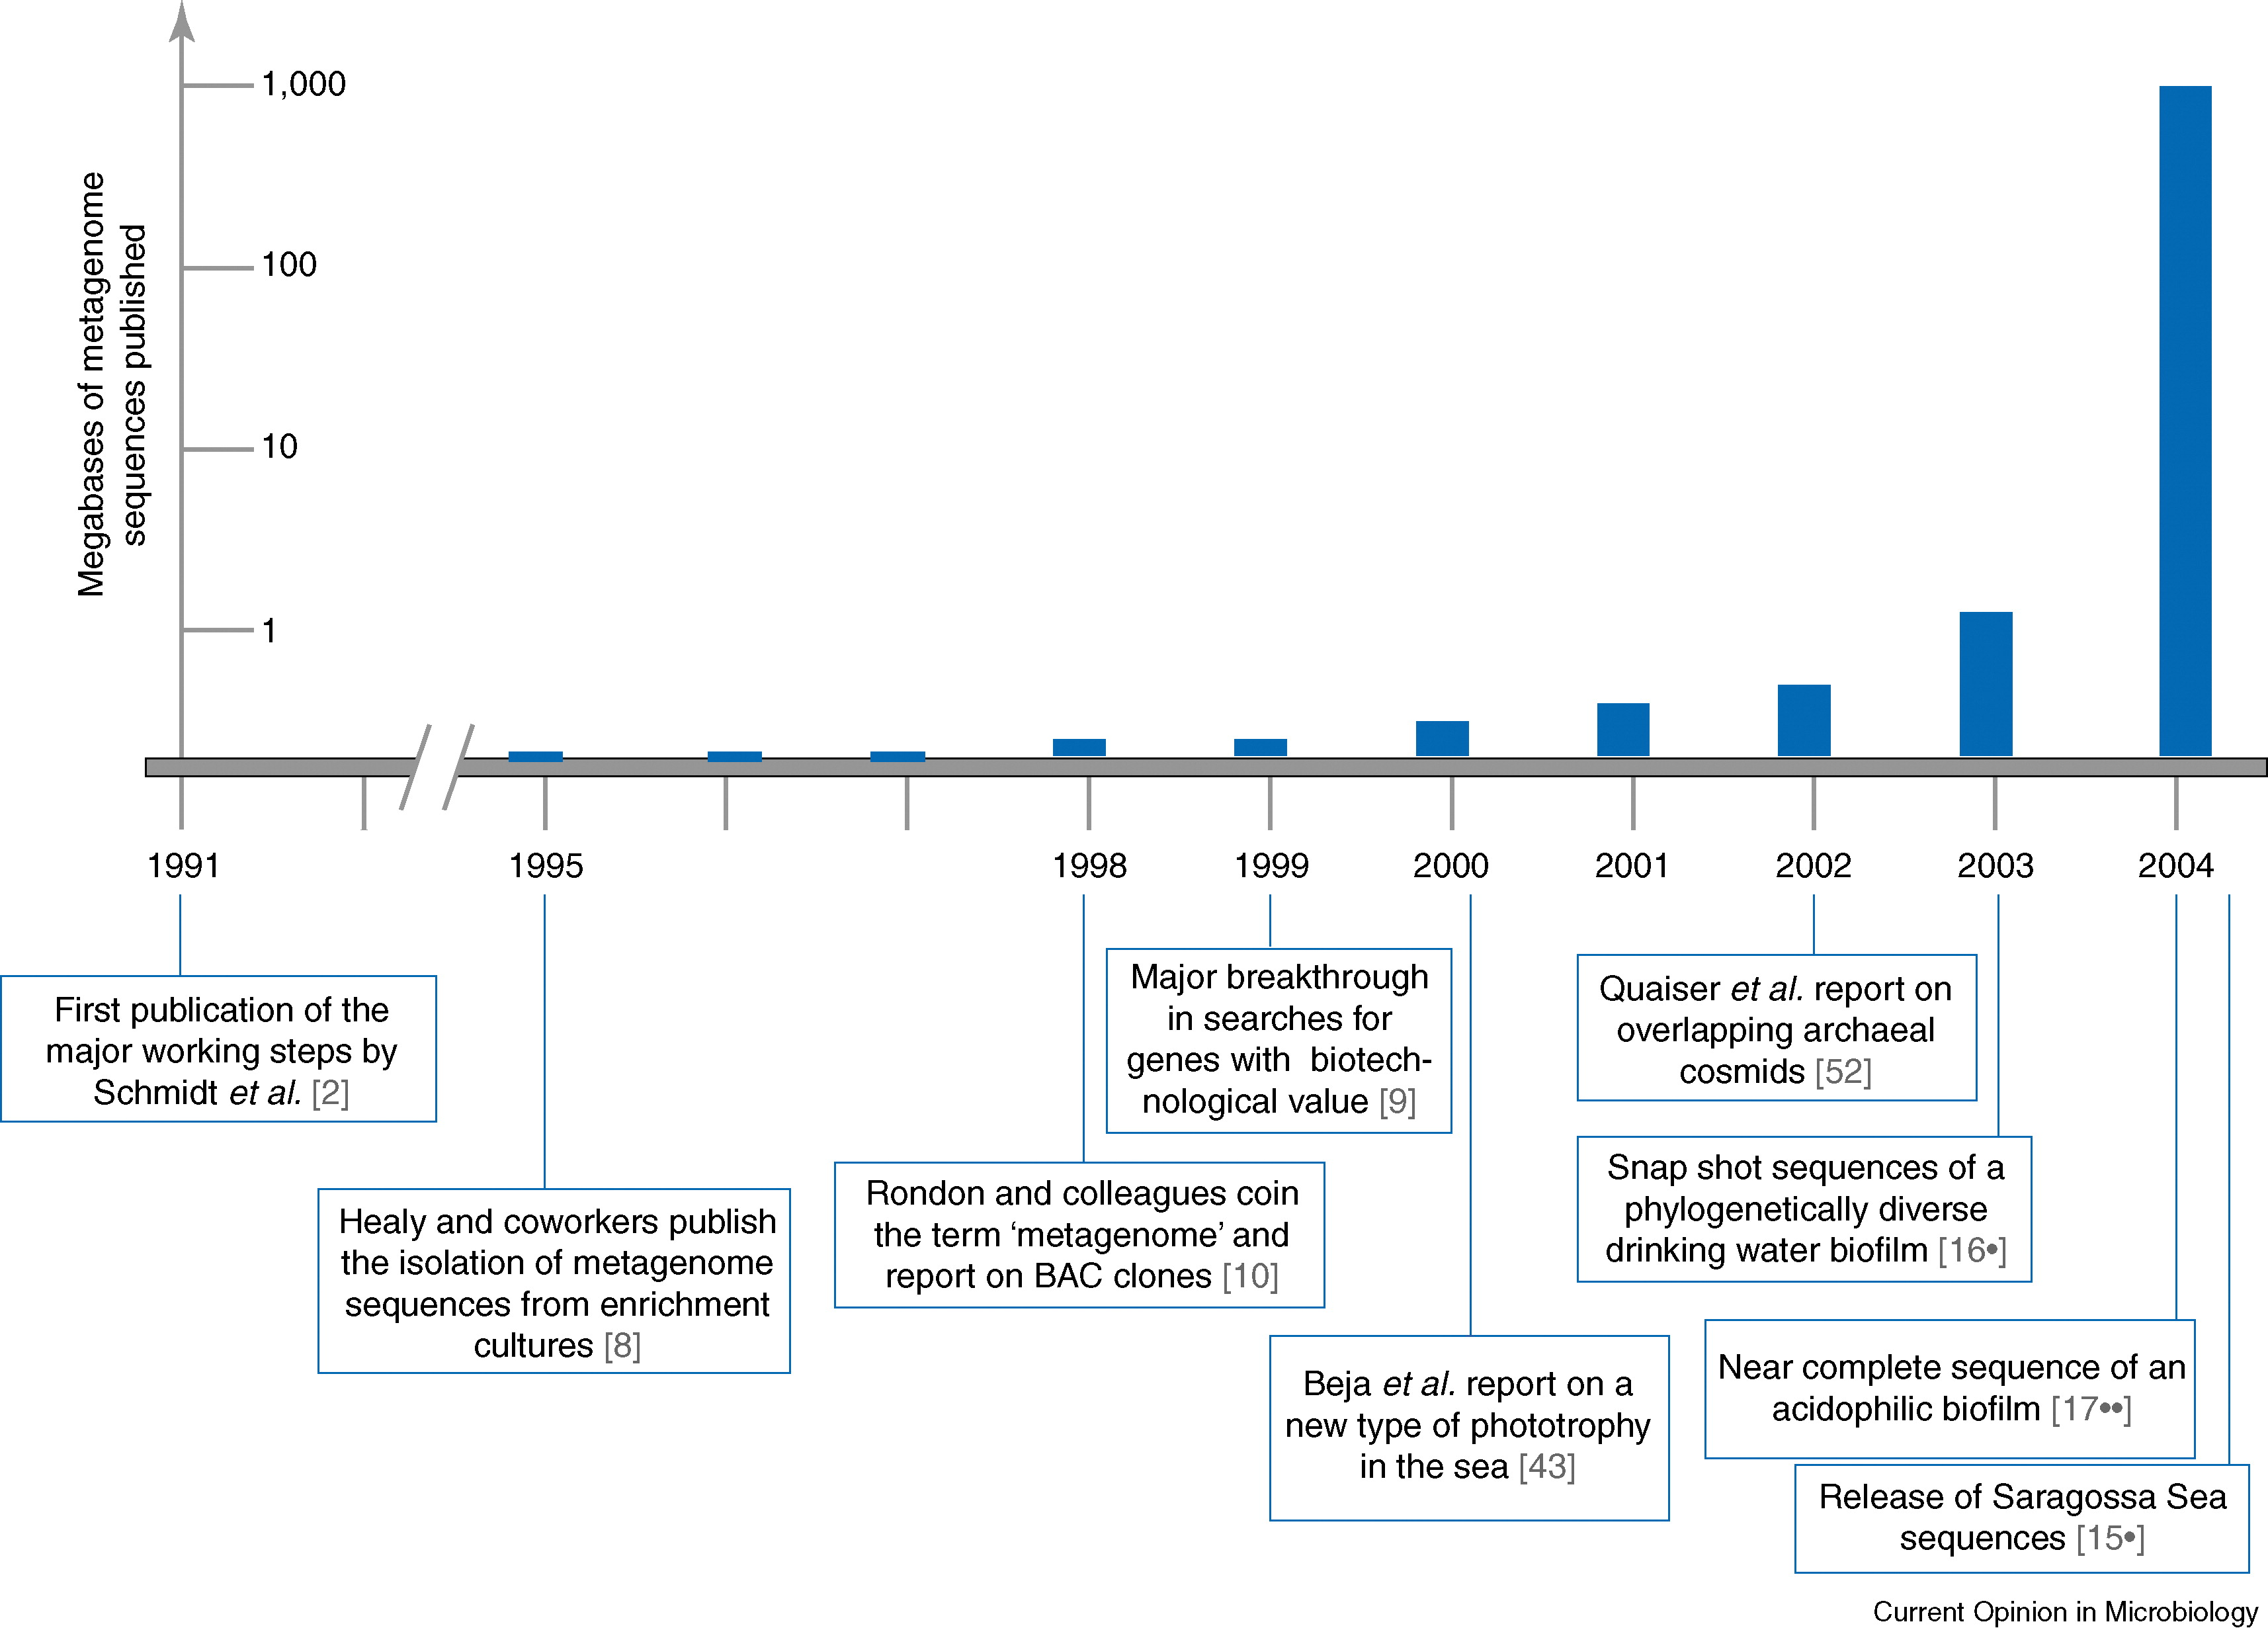
\includegraphics[width=.9\linewidth]{bilder/growth_of_novel_gene_discovery.jpg}	
%\caption{Timescale of metagenomic-derived and published DNA sequences. The timescale ranges from 1991, the initial outline of the major working steps, to the first mapping of archaeal comids in 2002 and the snap shot sequence analysis of the Sargasso Sea %published earlier this year.--taken from Streit \textit{et al.} \cite{STREIT2004492} just for comparison of published DNA sequences -- single events are not of importance for this}
%\label{img:nov_gene_discov}
%\end{figure}
\subsection*{Metagenomics analysis}
\paragraph*{Alignment-based methods}
The popular approach to analyze reads are the various alignment-based methods.\\
Sequences are aligned against a database of known transcripts, the resulting profiles are analyzed based on several factors.\\
This approach is well established and implemented numerous times. BLAST for example has an accuracy well over 80\%\cite{doi:10.1142/9789814295291_0003}  and similar values are expected for other alignment-based tools. Still BLAST is not used for metagenomics anymore due to low speed.\\
However, NGS supplies researchers with a lot of data to be analyzed. The analysis of metagenomes is computation heavy. BLAST, and therefore BLAST-like tools, aligns queries with the entries in a database. Applied on metagenomic data this method can be time consuming.\\
Research of  novel sequences is a main focus of metagenomics. This data stays unanalyzed following an alignment-based approach, resulting in a high demand for lightweight tools independent of databases.
\paragraph*{}
Here, I will showcase methods with differed approaches to the analysis of such data. 
\subsection*{An alternative for alignment-based methods}
The work of Song \textit{et al.} \cite{doi:10.1093/bib/bbt067} and Laczny \textit{et al.} \cite{Laczny2014} utilizes statistics, and visualization and machine learning for alignment-free approaches of analysis, respectively.\\
The statistical methods stated by Song \textit{et al.} are on their own inapt to analyze metagenomes, as they examine the similarity of two sequences. After application to every pair of sequences, a similarity or dissimilarity matrix is achieved. This can then be used for clustering or visualization.\\
Laczny \textit{et al.} utilizes a number of tools to construct a promising approach to alignment-free analysis.
%Apart from alignment of sequences another way is basing the analysis on different factors associated with metagenomic data. In this report I reflect the work of Song \textit{et al.} \cite{doi:10.1093/bib/bbt067} and Laczny \textit{et al.} \cite{Laczny2014} both presenting methods for the analysis of metagenomic-data using alignment-free approaches. Their work is based on statistical methods, and visualization and machine learning respectively.
\section*{Methods}
In this section "power" refers to the statistical term, which is the probability that a test correctly rejects the null hypothesis. With $H_0$: the sequences are unrelated; and $H_1$: the sequences are related under the underlying model. If not stated differently.
\subsection*{$k$-tuples as a measure of similarity}
Song \textit{et al.}\cite{doi:10.1093/bib/bbt067} present different methods based on $k$-tuple occurrences in sequences. A $k$-tuple is a substring of length $k$.\\
By counting the occurrences of these $k$-tuples and applying a distance or dissimilarity metric, the k-tuples are clustered and these clusters analyzed. Different metrics are stated as statistics, which are a function of two sequences, computing the similarity of those.\\
\paragraph*{The $D_2$ statistic}
Torney \textit{et al.}\cite{torney1990computation} introduced $D_2$  using shared $k$-tuple  occurrences between sequences to define similarity.
$$D_2=\sum_{w\in \mathcal{A}^k}X_wY_w$$
where $X_w$ and $Y_w$ are the numbers of occurrences of string $w$ in the corresponding sequence $A$ or $B$, $ \mathcal{A}$ is the alphabet and $k$ is the length of $w$.\\
Kantrovitz \textit{et al.}\cite{kantorovitz2007statistical} stated that the $D_2$ statistic depends on the  underlying sequence model and performed a normalization to remove the bias. A sequence model describes the different background probabilities of the observed sequences $A$ and $B$, here Markov models are used.
The resulting statistic is called $D2z$ and is defined as
$$D2z(A,B)=\frac{D_2(A,B)-E(D_2)}{\sqrt{Var(D_2)}}$$
The expected value and variance are calculated through consideration of background Markov models for the sequences.\\
$D2z$ was compared to five other measures of similarity -- \cite{doi:10.1093/bib/bbt067,kantorovitz2007statistical} -- through analysis of $cis$-regulatory modules (CRM), outperforming all of them. However $D2z$ requires two parameters; $k$ and $r$, where $k$ is the length of $w$ and $r$ is the order of the sequence Markov chain. The order of a MC states the dependence of the probability on the $r$ previous states. A MC of order zero is just the probability of a state, while a MC of order 1 is the probability of the last state given the previous state $P(w_n|w_{n-1}\dots w_1)=P(w_n|w_{n-1})$
\paragraph*{Expected value using Markov models}
For these calculations the order of the Markov chain is essential.\\
Generally the expected value $E(D_2)$ is the probability that the sequences are identical for a word of length $k$. \\
For a MC of $r$=0 this is equal to  the sum of the background probabilities $f_a^A$ $f_a^B$ to the power of $k$, where $a$ is the letter .
$$E(D_2)=P(I(A=B)=1)=\left(\sum_{a \in \mathcal{A}}f_a^Af_a^B\right)^k$$
where $I$ is the indicator function.\\
For a MC with $r$=1, $E(D_2)$ is the sum of all probabilities of words with length $k$. $$\sum_{|w|=k}P^A(w)P^B(w)$$
where $P^A(w)=p^A(w_1)p^A(w|w_1)$ (for $B$ analogous). Since $r=1$ the probability is given by the probability for the first letter multiplied by the probability of the word given the first letter. Similar calculations can be done for MC of higher order.\\
The calculation of the variance relies on its relationship with covariance, further insight into this is given in \cite{kantorovitz2007statistical}.
\paragraph*{Phylogenetic trees through statistics -- CVTree}
Another approach utilizes the expected count of a $k$-tupel under the $(k-2)$-th order Markov chain, estimated by 
$$E_w^X=\frac{X_wX_{w_2\dots w_k}}{X_{w_2\dots w_{k-1}}}$$
where $w$ is a substring of length $k$, $w_i$ is the letter at index $i$ in $w$ and $X_w$ is the number of occurrences of $w$ in a sequence $A$.\\
The correlation coefficient of the relative difference vectors with the expected count is then used to measure similarity of sequences\cite{doi:10.1093/bib/bbt067}.
$$Hao=\frac{1}{2}\left(1-C\right)$$
\\
$Hao$ calculates the frequencies of observations of overlapping $k$-tupels indicated with $X_w$ in a composition vector and subtracts a random background using the $(k-2)$-th order Markov chain. This step is similar to the normalization in $D2z$ and is to minimize the influence of random mutation. After computation of correlation $C$ a normalization was defined by subtraction of $C$ from 1 and multiplication with $.5$.
$$C=\frac{\sum_w\left(\frac{X_w-E_w^X}{E_w^X}\right)\left(\frac{Y_w-E_w^Y}{E_w^Y}\right)}{\sqrt{\sum_w\left(\frac{X_w-E_w^X}{E_w^X}\right)^2\sum_w\left(\frac{Y_w-E_w^Y}{E_w^Y}\right)^2}}$$
$C$ describes the cosine of the angle between the composition vectors of the sequences, where $C=1$ $\Leftrightarrow A=B$ and $C=0$ $\Leftrightarrow \forall a_i \in A,$ $b_i \in B:$ $a_i \neq b_i$. \\
For CVTree a distance matrix is computed by applying $Hao$'s method to each pair of sequences. Neighbor joining is then used to construct a phylogenetic tree.\\
CVTree was tested by Qi \textit{et al.} on a set of 139 prokaryotic genomes computing a robust result\cite{qi2004cvtree}. \\
The application of CVTree on virus data, provided on the web service, shows the relationship of the provided data (Figure \ref{img:cvtree}).
\begin{figure*}
	\centering
	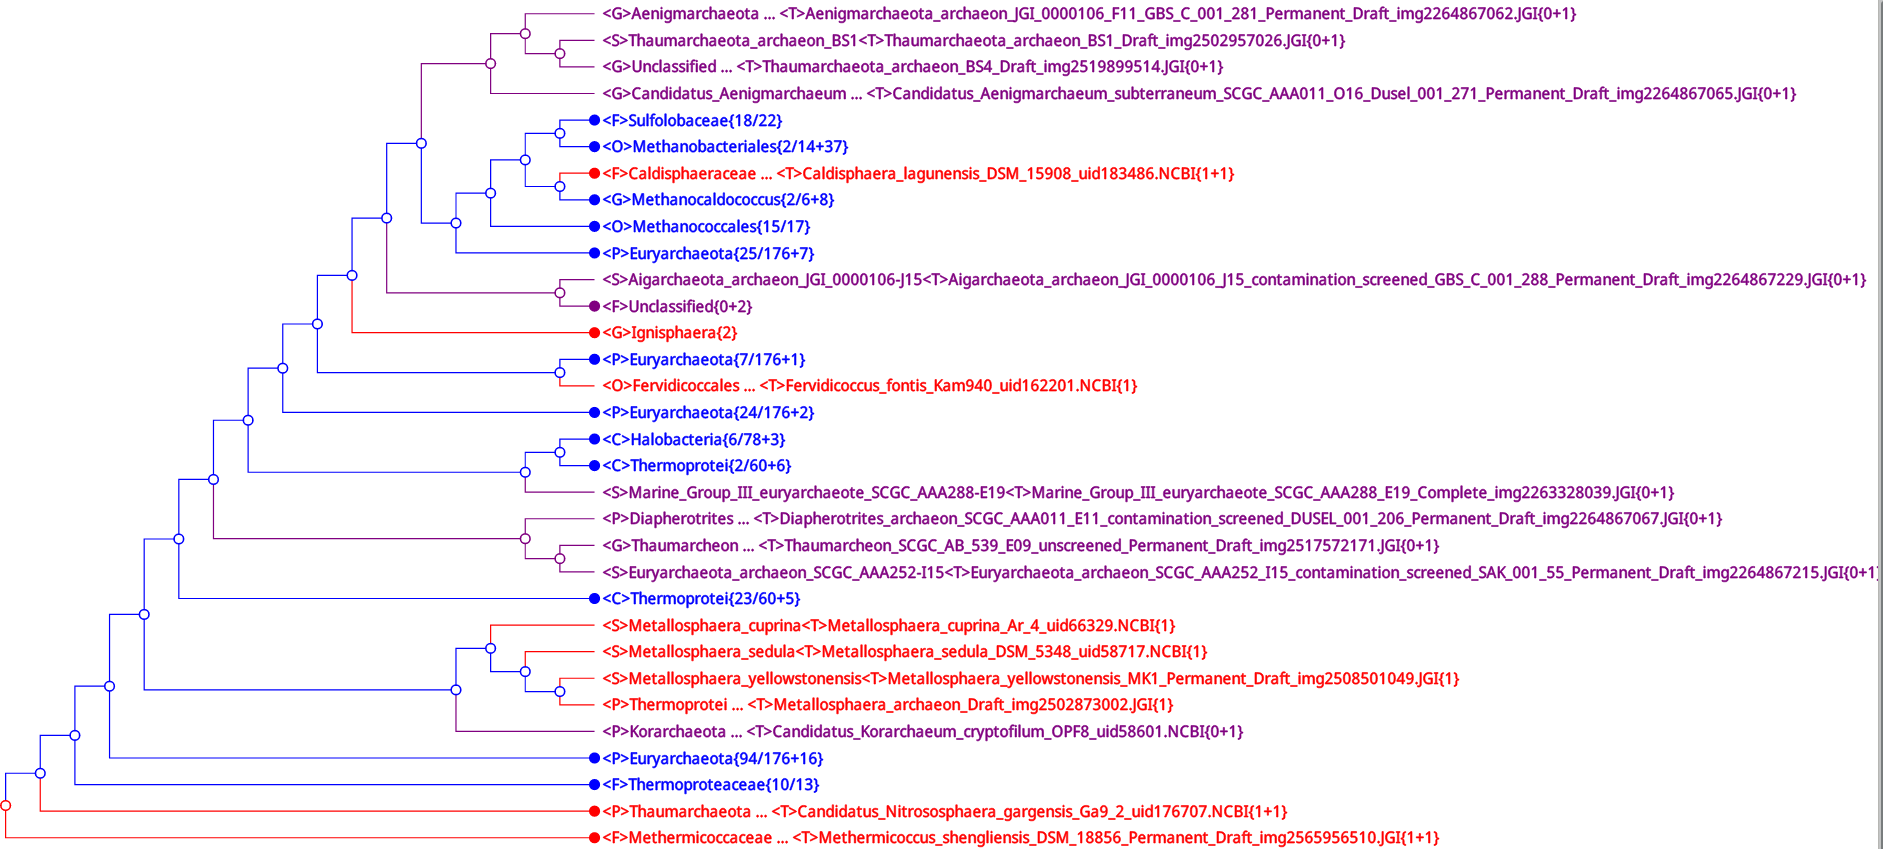
\includegraphics[width=.99\textwidth]{bilder/CVTree.png}
	\caption{Example run of CVTree with Virus data and $k=6$ executed with web service at\newline \url{http://tlife.fudan.edu.cn/archaea/cvtree/cvtree3/} \cite{qi2004whole,zuo2015cvtree3}}
	\label{img:cvtree}
\end{figure*}%
\paragraph*{Similarity through nucleotide frequency}
A related approach was presented by Karlin and colleagues, where they observed the relative di-nucleotide frequency defined by $$\rho_{ab}(A)=\frac{f_{ab}}{f_af_b}$$
where $f_w$ is the frequency of $w$ in a sequence.\\
It is stated that $\rho_w$ is stable across a genome and differs in different genomes. The extension to tri- and tetra-nucleotides is achieved by $$\gamma_{abc}=\frac{f_{abc}f_af_bf_c}{f_{ab}f_{bc}f_{aNc}}$$
and 
$$\tau_{abcd}=\frac{f_{abcd}f_{ab}f_{aNc}f_{aN_1N_2d}f_{bc}f_{bNd}f_{cd}}{f_{abc}f_{abNd}f_{bcd}f_af_bf_cf_d}$$
$l_p$ norm was applied as a dissimilarity measure as
$$\delta(A,B)=\sum_{j\in A}|\theta_j(A)-\theta_j(B)|$$
where $A$, $B$ are sequences, $\theta \in \{\rho, \gamma, \tau\}$ and
$$j=\begin{cases}
\{a,b\} &\textrm{ if }\theta=\rho\\
\{a,b,c\} & \textrm{ if }\theta=\gamma\\
\{a,b,c,d\} &\textrm{ if }\theta=\tau
\end{cases}$$
Evolutionary studies on viruses, bacteria, plasmids, prokaryotes and eukaryotes were performed using this measure\cite{doi:10.1093/bib/bbt067}.
\paragraph*{$D_2^S$, $D_2^*$, $d_2^S$ and $d_2^*$}
The $D_2^S$ statistic is defined by
$$D_2^S=\sum_{w\in \mathcal{A}^k}\frac{\widetilde{X}_w\widetilde{Y}_w}{\sqrt{\widetilde{X}_w^2+\widetilde{Y}_w^2}}$$
where $\widetilde{X}_w$ and $\widetilde{Y}_w$ are the normalization of $X_w$ and $Y_w$ respectively
$$\widetilde{X}_w=X_w-\bar{n}p_w^X$$
$\bar{n}=n-k$ and $p_w^X$ is the probability of the  $k$-tupel $w$ under the background model of a sequence $A$.
This is based on Shepp\cite{shepp1962normal}. Where it was observed that for two normal random variables with mean zero, $XY/\sqrt{X^2+Y^2}$ is also normally distributed.\\
$D_2^*$ defined by
$$D_2^*=\sum_{w\in \mathcal{A}^k}\frac{\widetilde{X}_w\widetilde{Y}_w}{\sqrt{\bar{m}\bar{n}p_w^Xp_w^Y}}$$
utilizes the idea that the number of occurrences of $w$ is approximately Poisson distributed and mean and variance are the same.\\
Through simulations and theoretical studies the null hypothesis $H_0$ was tested against $H_1$; the conclusions were:
\begin{enumerate}
\item 	$D_2^S$ and $D_2^*$ have higher power than $D_2$ increasing with sequence length
\item $D_2^*$ has the highest power when the length of $k$ equals the $motif$ length
\item For short sequences the power of $D_2^*$ is higher while for long sequences $D_2^S$ is generally more powerful.
\end{enumerate}
Here $motifs$ are significantly enriched word patterns \cite{doi:10.1093/bib/bbt067}.\\
\\
Further normalization of $D_2^S$ and $D_2^*$ removes the property that the magnitude strongly varies depending on different factors. The resulting statistics are $d_2^S$ and $d_2^*$ respectively.
$$d_2^S=\frac{1}{2}\left(1-\frac{D_2^S}{\sqrt{\frac{\sum_{w\in \mathcal{A}^k}\widetilde{X}_w^2}{\sqrt{\widetilde{X}_w^2+\widetilde{Y}_w^2}}}\sqrt{\frac{\sum_{w\in \mathcal{A}^k}\widetilde{Y}_w^2}{\sqrt{\widetilde{X}_w^2+\widetilde{Y}_w^2}}}}\right)$$
and
$$d_2^*=\frac{1}{2}\left(1-\frac{D_2^*}{\sqrt{\frac{\sum_{w\in \mathcal{A}^k}\widetilde{X}_w^2}{\bar{n}p_w^X}}\sqrt{\frac{\sum_{w\in \mathcal{A}^k}Y_w^2}{\bar{m}p_w^Y}}}\right)$$
$d_2^S$ and $d_2^*$ now hold the property that they are 0 when the sequences are the same and close to 1 if they are anti-correlated.
Through this $d_2^S$ and $d_2^*$ can be used to cluster sequences of interest. 
\paragraph*{Modification of $d_2^S$ and $d_2^*$}
The statistics mentioned above consider exact matches of tupels, since mutations are a fundamental part of evolution and DNA replication in general, mismatches should be considered when applying these methods. For a tupel $w$ its neighborhood can be defined as $\varsigma(w)$ with $w' \in \varsigma(w)$ when $w'$ has up to a certain number of mismatches with $w$ and a weight $a$ is applied, analogously reverse complements can be included in $\varsigma(w)$.\\
The statistics are modified as $\widetilde{X}_w$ is replaced by $\widetilde{X}_{\varsigma(w)}$ where $\widetilde{X}_{\varsigma(w)}=X_{\varsigma(w)}-EX_{\varsigma(w)}$ and 
$$X_{\varsigma(w)}=\sum_{w'\in\varsigma(w)}a_{w'}X_{w'}$$ 
modifications for $\widetilde{Y}_w$ are analogous.
Song \textit{et al.} performed a series of tests to evaluate the effectiveness of the statistics $Hao$, $d_2^S$ and $d_2^*$ with consideration of mismatches. The neighborhood was defined as $$\varsigma(w)=\{w',rc(w')|dist_{hamming}(w,w')\leq 1\}$$
Testing was based on sequences taken from mouse embryos. The positive set was taken from the forebrain, midbrain, limb and heart tissues, while the negative set was chosen from random samples of the same length with a maximum of 30\% repetitive sequences \cite{doi:10.1093/bib/bbt067}.\\
For 500 samples of each set the dissimilarity was calculated for each pair in the respective set. A threshold for dissimilarity was applied on the resulting values, a score lower than the threshold was predicted as positive, one above indicated negatives. Through comparison with the real data false predictions were identified.\\
Different parameters like tupel size $k$, Markov chain order and mismatch weight were applied.
\paragraph*{Performance under the mismatch model}
Conclusions of these test were: 
\begin{enumerate}
\item $Hao$ performed worse than both $d_2^S$ and $d_2^*$	
\item $d_2^S$ and $d_2^*$ performed best with $k=4$ and mismatch weight of around 0.05. However differences through mismatch weight were negligible. For $k=5 \lor 6$ a weight close to 1 performed best.
\end{enumerate}
Song \textit{et al.} considered additional statistics for testing, which are not discussed in this report and were therefore not further accounted for.\\
\\
Additional testing using metagenomes and NGS data was carried out \cite{doi:10.1093/bib/bbt067}, since usually the short reads generated through NGS reduce the power of the discussed statistics. The data consisted of 39 fecal samples of 33 mammalian hosts \cite{muegge2011diet} 56 marine samples \cite{rusch2007sorcerer} and 13 human fecal samples \cite{kurokawa2007comparative} for metagenomes and tree species with unknown complete genomes as NGS data.\\
$d_2^S$ outperformed the other tested measures in terms of consistency and separation as was seen through the tree samples and human feces metagenome respectively \cite{doi:10.1093/bib/bbt067}. \\
Overall $d_2^S$ produced the best results compared to all mentioned statistics with $Hao$ and $d_2^*$ having similar outcomes.
\subsection*{Machine learning}
In his work van der Maaten \cite{DBLP:journals/corr/abs-1301-3342} introduced a machine learning variant (BH-SNE ) based on the observation that closely related objects induce a larger force upon each other than unrelated ones. While these objects were originally intended to be points in a picture, Laczny \textit{et al.}\cite{Laczny2014} used reads from metagenomes.\\
Barnes-Hut-SNE applies the Barnes-Hut algorithm and metric trees to modify the t-SNE method.
\paragraph*{Barnes-Hut and vantage-point trees}
The Barnes-Hut algorithm is often used by astronomers to perform $N$-body simulations\cite{DBLP:journals/corr/abs-1301-3342}. In this algorithm it is assumed that the force of objects with sufficient large distance to each another is infinitesimal and thus can be ignored in further computation. Leading --in the case of BH-SNE -- to a decrease in objects to include in calculations.\\
Van der Maaten chose these objects based on vantage-point trees, where similar nodes are saved as the left and dissimilar nodes as the right child. After establishing the data structure one can search the tree and apply a given algorithm to the reduced set of nodes of interest. \\
\paragraph*{Sequence signatures as objects}
Observations suggest the existence of species-specific oligonucleotide signatures in genomic sequences\cite{Laczny2014,Cheng1194}. These consist of $k$-mers and can be represented as vectors in high-dimensional Euclidean space. For human interpretation these vectors need to be transformed in a two or three dimensional space \cite{Laczny2014}.\\
vector construction is achieved through assignment of joint probabilities to the $k$-mers and a similarity function to the corresponding points in high-dimensional space. Utilizing a Kullback-Leibler divergence and the optimizations stated before the points can be optimized.\\
Using center log-ratio (CLR)-transformation as a normalization, oligonucleotide signatures and the BH-SNE approach of van der Maaten, Laczny \textit{et al.} constructed a tool for application on metagenomic-data with sequence length of 1kb and 5-mers as oligonucleotide signatures. While these parameters produced the best results Laczny\textit{et al.} stated that 600 nt might be sufficient for some applications, but with lower values the separation of points would drop remarkably, as can be seen in Figure  \ref{img:seperation} through lesser separation of the clusters. Implementing their approach using 5-mers produced better congruency compared to transformed and untransformed 4-mers.\\
For Laczny \textit{et al.} these 5-mers are the objects, used for calculation of similarity in BH-SNE.
\begin{figure}[p]
	\centering
	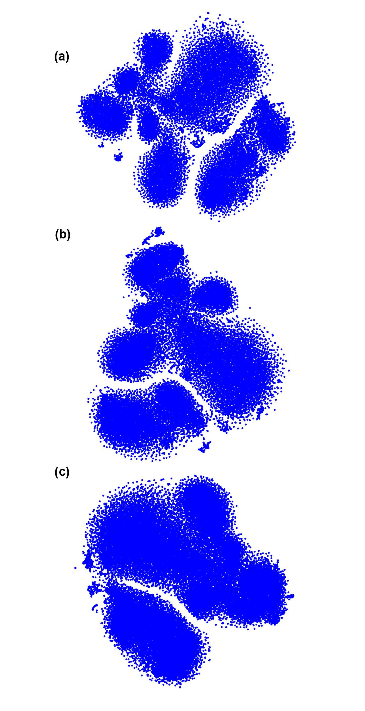
\includegraphics[width=.6\linewidth]{bilder/seperation.png}
	\caption{BH-SNE-based visualization of genomic fragment signatures for
		EqualSet01 (even community, overall reflecting distant taxonomic relatedness) with varying
		fragment lengths.
		(a) 800nt.  (b) 600nt.  (c) 400nt. -- from Laczny \textit{et al.}\cite{Laczny2014}}
	\label{img:seperation}
\end{figure}%
\paragraph*{Clustering}
The tool was tested on several simulated data sets; EqualSet01,EqualSet02 and LogSet01. The genomes of organisms in these sets were equally and logarithmically distributed; among the equally distributed sets were genomes with small and high similarity respectively. \\
They consisted of ten organisms depicted in Table \ref{tab:eqloggenes} for EqualSet01 and LogSet01, and Table \ref{tab:eqgenomes} for EqualSet02.
\begin{table*}
	\centering
	\caption{Genomes of EqualSet01 and LogSet01 \cite{Laczny2014}}
	\begin{tabular}{ccc}
		Organism&Genome size (nt)&\%GC\\
		\textit{Leifsonia xyli} subsp.  xyli str.  CTCB07&2,584,158&67.7\\
		\textit{Escherichia coli} UTI89&5,065,741&50.6\\
		\textit{Candidatus}	Carsonella ruddii PV&159,662&16.6\\
		\textit{Haemophilus influenzae}	PittGG&1,887,192&38.0\\
		\textit{Bacillus amyloliquefaciens}	FZB42&3,918,589&46.5\\
		\textit{Brachyspira hyodysenteriae} WA1&3,000,694&27.1\\
		\textit{Geodermatophilus obscurus} DSM 43160&5,322,497&74.0\\
		\textit{Rickettsia prowazekii} str.  Dachau&1,109,051&29.0\\
		\textit{Escherichia coli} str.  ’clone D i14’&5,038,386&50.6\\
		Uncultured Termite group 1 bacterium phylotype Rs-D17&1,125,857&35.2	
	\end{tabular}
\label{tab:eqloggenes}
\end{table*}
\begin{table*}
	\centering
	\caption{Genomes of EqualSet02 \cite{Laczny2014}}
	\begin{tabular}{ccc}
		Organism&Genome size (nt)&\%GC\\
		\textit{Lactobacillus delbrueckii} subsp.  bulgaricus ATCC 11842&1,864,998&49.7\\
		\textit{Lactobacillus brevis} ATCC 367&2,291,220&46.2\\
		\textit{Lactobacillus casei} ATCC 334&2,895,264&46.6\\
		\textit{Lactobacillus gasseri}	ATCC 33323&1,894,360&35.3\\
		\textit{Shewanella amazonensis}	SB2B&4,306,142&53.6\\
		\textit{Shewanella putrefaciens} CN-32&4,659,220&44.5\\
		\textit{Shewanella baltica}	OS195&5,347,283&46.3\\
		\textit{Shewanella frigidimarina}	NCIMB 400&4,845,257&41.6\\
		\textit{Streptococcus suis}	A7&2,038,409&41.2\\
		\textit{Streptococcus thermophilus}	CNRZ1066 chromosome&1,796,226&39.1
	\end{tabular}
\label{tab:eqgenomes}
\end{table*}%
The equally distributed data set is simplistic. As real-world metagenomes are never evenly distributed. The logarithmic set should simulate this real-world data with varying quantities of different genomes. High and low similarity sets test the discrimination capabilities of the tool.\\
After applying their tool on the simulated metagenomes their results showed distinct clustering for different species as depicted in Figure \ref{img:clusterData1} for EqualSet01 and LogSet01, respectively. Clustering of EqualSet02 resulted in overlapping of closely related organisms and separation of more distant relatives. \\
Overall the runs on simulated data resulted in high sensitivity, specificity and accuracy(Table \ref{tab:sens-spec-acc1}). The calculation was performed by enclosing clusters with polygons, by hand, as seen in Figure \ref{img:clusterData1}. Points inside represent the positives, points outside the negatives. Similar outputs were achieved by fitting (semi-~)automated Gaussian Mixture models to calculate these values.
\begin{figure}[p]
	\centering
	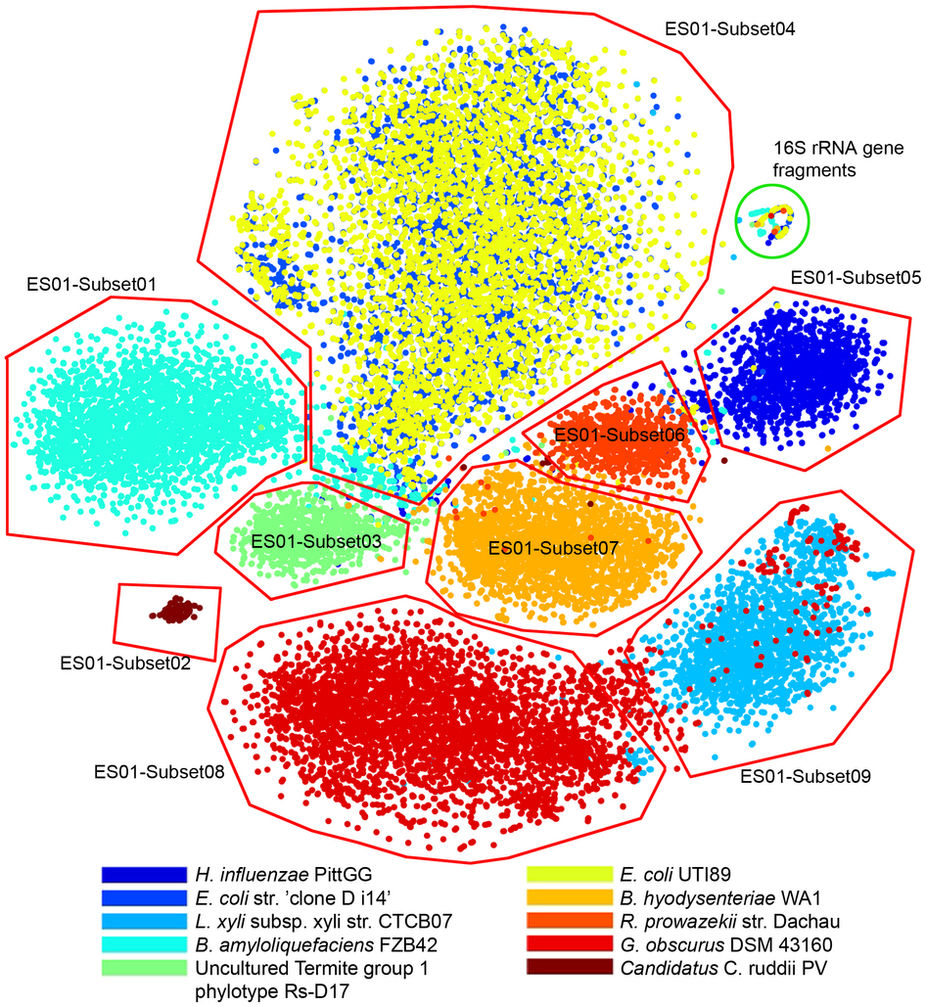
\includegraphics[width=.98\linewidth]{bilder/clusterData1.jpg}
	\caption{Figure taken from Laczny \textit{et al.} \cite{Laczny2014} where red polygons mark clusters of congruent sets of interest used for calculation of sensitivity, specificity and accuracy. Colors mark different organisms as seen in the legend. The green polygon marks the cluster of 16s rRNA, forming a distinct group}
	\label{img:clusterData1}
\end{figure}%
\begin{table*}[h]
	\centering
	\caption{Sensitivity, specificity and accuracy of EqualSet01 -- excerpt from Laczny \textit{et al.}\cite{Laczny2014}}
	\begin{tabular}{c|c|c|c|c}
		Subset&Sensitivity (\%)&Specificity(\%)&Accuracy(\%)&Organism\\
		\hline
		01&90.06&99.99&99.94&B. \textit{amyloliquefaciens}\\
		02&91.25&100&100&\textit{Candidatus} C. ruddii\\
		03&95.42&99.90&97.57&Uncultured Termite group1 bacterium\\
		04&98.60&98.23&96.67&E. \textit{coli}
	\end{tabular}
\label{tab:sens-spec-acc1}
\end{table*}%
\paragraph*{Application on real-world metagenomes}
Testing on real-world metagenomes of ground water \cite{Wrighton1661}, the human gut \cite{Arumugam2011} and the deep sea \cite{Konstantinidis15082009} was also performed. They reported similar clustering (Figure \ref{img:humangut}) compared to simulated data with sensitivity, specificity and accuracy well above 90\% for all subsets of the human gut metagenome with one exception, where accuracy was slightly below 80\%.\\
The values were calculated using polygons to mark clusters and verifying these by comparison with the NCBI non-redundant nucleotide database.\\
The ground water metagenome also produced distinct clusters (Figure \ref{img:groudwater}). Calculation of sensitivity, specificity and accuracy could not be carried out since they reported a lack of characterized reference genomes. Instead they used what they called "essential genes" which can indicate the completeness of a genome. They reported four out of eight of these essential genes as over 80\% complete, indicating a positive result for their tool.\\
As for the marine sample, the clusters, as seen in Figure \ref{img:deepsea}, identified by the tool were linked to yet  uncharacterized data.
	\begin{figure}[p]
		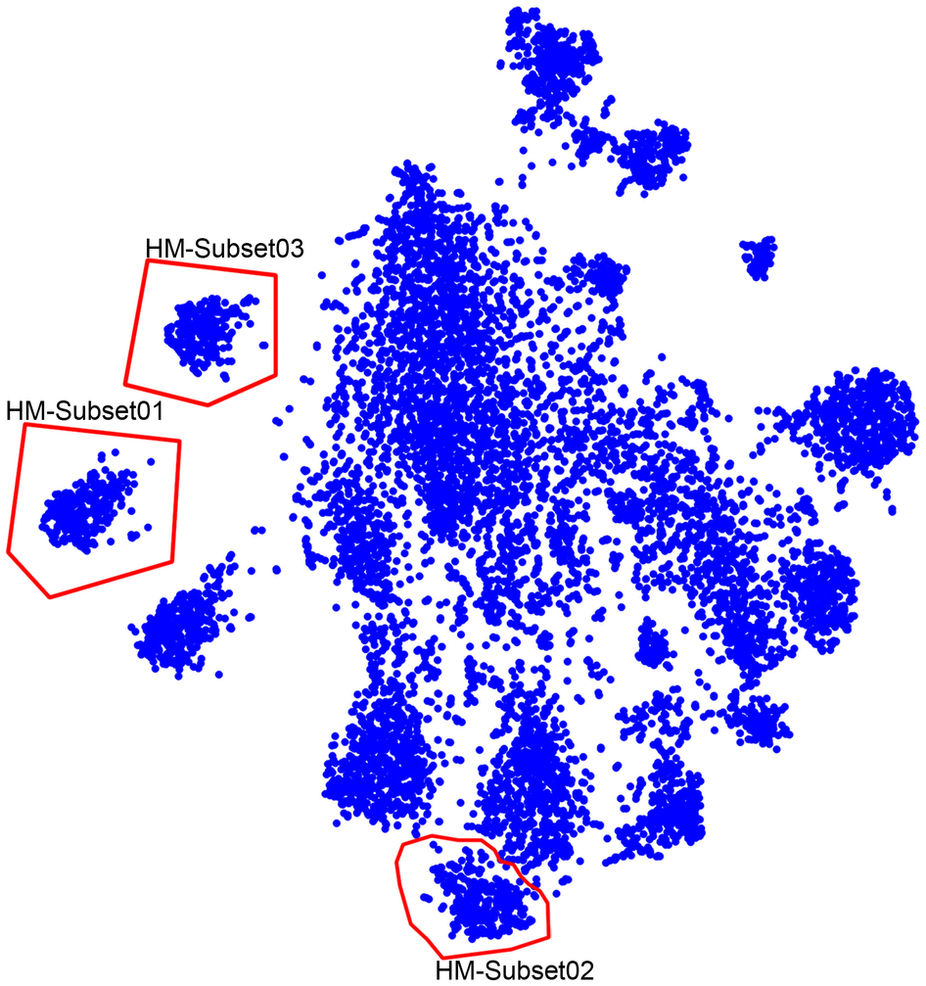
\includegraphics[width=.9\linewidth]{bilder/humangutCluster.jpg}
		\caption{Clustering of human gut metagenome. Polygons represent clusters of great interest -- from Laczny \textit{et al.}\cite{Laczny2014}}
\label{img:humangut}	
\end{figure}%
	\begin{figure}[p]
		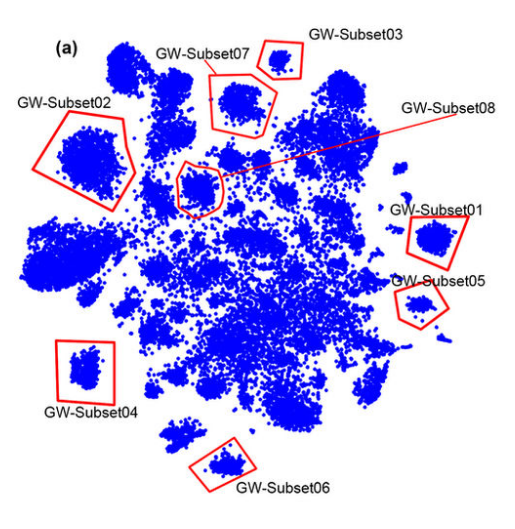
\includegraphics[width=.9\linewidth]{bilder/groudwaterCluster.png}
		\caption{Clustering of groud water metagenome. Polygons represent clusters of great interest -- from Laczny \textit{et al.}\cite{Laczny2014}}
		\label{img:groudwater}
	\end{figure}%
\begin{figure}[h]
		\centering
	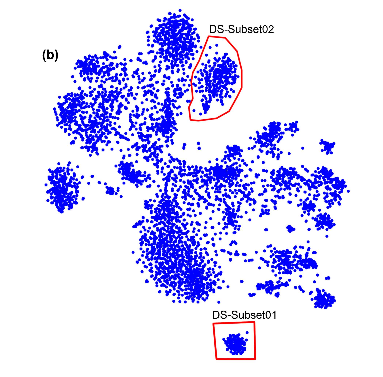
\includegraphics[width=.9\linewidth]{bilder/marineCluster.png}
	\caption{Clustering of deep sea metagenome. Polygons represent clusters of great interest -- from Laczny \textit{et al.}\cite{Laczny2014}}
	\label{img:deepsea}
\end{figure}%

Compared to an ESOM-based approach, tested with the same data sets, Laczny \textit{et al.} reported better clustering of metagenomic-data. Additionally also a significant reduction in runtime \cite{Laczny2014} for their used metagenomes and good visualization capabilities as tested on simulated and real-world data.\\
Clustering seems robust on the applied metagenomes, while similar data tends to be near to each other in the visualization, 16S rRNA sequences form a distinct cluster, due to the high conservation of these regions in the genome.\\
As a downside sequences of 1kb are required to achieve good clustering, which are yet hard to gather through raw reads. Advancements in sequencing technologies are needed to fully utilize the capabilities of this tool.
\section*{Conclusions}
The different methods for $k$-tuple counts and oligonuclotide signature enable an analysis independent on coding regions and fully sequenced genomes. This is of particular importance for the study of novel transcripts and a better understanding of mirobiotal organisms.\\
However, the statistics in Song \textit{et al.} have to be applied through a dissimilarity matrix to obtain meaningful results for metagenomic data, and rise in complexity as the power increases. This makes for slower computation of statistics like $d_2^S$ compared to $D2z$. For new methods the results have to be normalized, as otherwise they are not comparable in metagenomic context.\\
While Laczny \textit{et al.}'s approach delivers good results for the tested metagenomes it is not clearly defined which clusters are of real significance and which can be ignored in further research. Without additional data, all clusters visible in the plot have to be analyzed manually. However, a general foundation of relationship is still established.\\
Furthermore I was not able to test any of the tools myself. This was due to different factors. While Laczny \textit{et al.} state the steps leading to the construction of the tool, it is not publicly available so a considerable amount of work is needed to correctly rebuilt it.\\
The statistics-tools are either out of date or poorly documented. It is not apparent what parameters are required or how the computation is achieved. More often than not a particular file type is required, resulting in conflicts with publicly available metagenomic data.\\
However, CVTree is still in development and a test run with provided data was successful (Figure \ref{img:cvtree}), the upload of custom data was not possible at the time.
%%%%%%%%%%%%%%%%
%% Background %%
%%
%\section*{Content}
%\section*{Section title}
%\subsection*{Sub-heading for section}
%\subsubsection*{Sub-sub heading for section}
%\paragraph*{Sub-sub-sub heading for section}

%%%%%%%%%%%%%%%%%%%%%%%%%%%%%%%%%%%%%%%%%%%%%%
%%                                          %%
%% Backmatter begins here                   %%
%%                                          %%
%%%%%%%%%%%%%%%%%%%%%%%%%%%%%%%%%%%%%%%%%%%%%%

\begin{backmatter}



%%%%%%%%%%%%%%%%%%%%%%%%%%%%%%%%%%%%%%%%%%%%%%%%%%%%%%%%%%%%%
%%                  The Bibliography                       %%
%%                                                         %%
%%  Bmc_mathpys.bst  will be used to                       %%
%%  create a .BBL file for submission.                     %%
%%  After submission of the .TEX file,                     %%
%%  you will be prompted to submit your .BBL file.         %%
%%                                                         %%
%%                                                         %%
%%  Note that the displayed Bibliography will not          %%
%%  necessarily be rendered by Latex exactly as specified  %%
%%  in the online Instructions for Authors.                %%
%%                                                         %%
%%%%%%%%%%%%%%%%%%%%%%%%%%%%%%%%%%%%%%%%%%%%%%%%%%%%%%%%%%%%%

% if your bibliography is in bibtex format, use those commands:
\bibliographystyle{bmc-mathphys} % Style BST file (bmc-mathphys, vancouver, spbasic).
\bibliography{bibliography}      % Bibliography file (usually '*.bib' )
% for author-year bibliography (bmc-mathphys or spbasic)
% a) write to bib file (bmc-mathphys only)
% @settings{label, options="nameyear"}
% b) uncomment next line
%\nocite{label}

% or include bibliography directly:
% \begin{thebibliography}
% \bibitem{b1}
% \end{thebibliography}

%%%%%%%%%%%%%%%%%%%%%%%%%%%%%%%%%%%
%%                               %%
%% Figures                       %%
%%                               %%
%% NB: this is for captions and  %%
%% Titles. All graphics must be  %%
%% submitted separately and NOT  %%
%% included in the Tex document  %%
%%                               %%
%%%%%%%%%%%%%%%%%%%%%%%%%%%%%%%%%%%

%%
%% Do not use \listoffigures as most will included as separate files

%\section*{Figures}
 
%%%%%%%%%%%%%%%%%%%%%%%%%%%%%%%%%%%
%%                               %%
%% Tables                        %%
%%                               %%
%%%%%%%%%%%%%%%%%%%%%%%%%%%%%%%%%%%

%% Use of \listoftables is discouraged.
%%
%\section*{Tables}

%%%%%%%%%%%%%%%%%%%%%%%%%%%%%%%%%%%
%%                               %%
%% Additional Files              %%
%%                               %%
%%%%%%%%%%%%%%%%%%%%%%%%%%%%%%%%%%%

%\section*{Additional Files}

%  \subsection*{Additional file 2 --- Sample additional file title}


\end{backmatter}
\end{document}
